

\section{User Interface}
\subsection{Authentifizierung}
Zur Authentifizierung der Benutzer wird der OAuth 2 Standard verwendet. Dieser erlaubt ein Login mit einem GitHub, FaceBook oder anderem Konto. Implementiert wurde dieser Standard auf der \acs{rest} Seite mit Hilfe von verschiedenen Django Plugins. 
Beispielsweise wurde python-social-auth verwendet um den Benutzer gegenüber diesen Diensten zu authentisieren. Die \acs{rest} Schnittstelle wird dann über einen Token gesichert.

\subsection{Transformationen erstellen}
Wir wollten das Erstellen einer Transformation so einfach wie möglich gestalten. Zu diesem Zweck haben wir uns früh dazu entschlossen einen Wizard zu schreiben, welcher die Aktion vereinfachen soll (\cref{fig:pd:tables_per_click}). In den frühen Phasen des Projektes war es notwendig den Wizard zu verwenden. In der gelieferten Beta-Version, kann der Wizard verwendet werden. Die Transformation kann auch über den manuellen Editor erstellt werden (\cref{fig:pd:wizard-manual}), dann müssen allerdings entweder die Tabellennamen bekannt sein, oder es kann nur ein Template erstellt werden.
\begin{figure}[H]
\centering
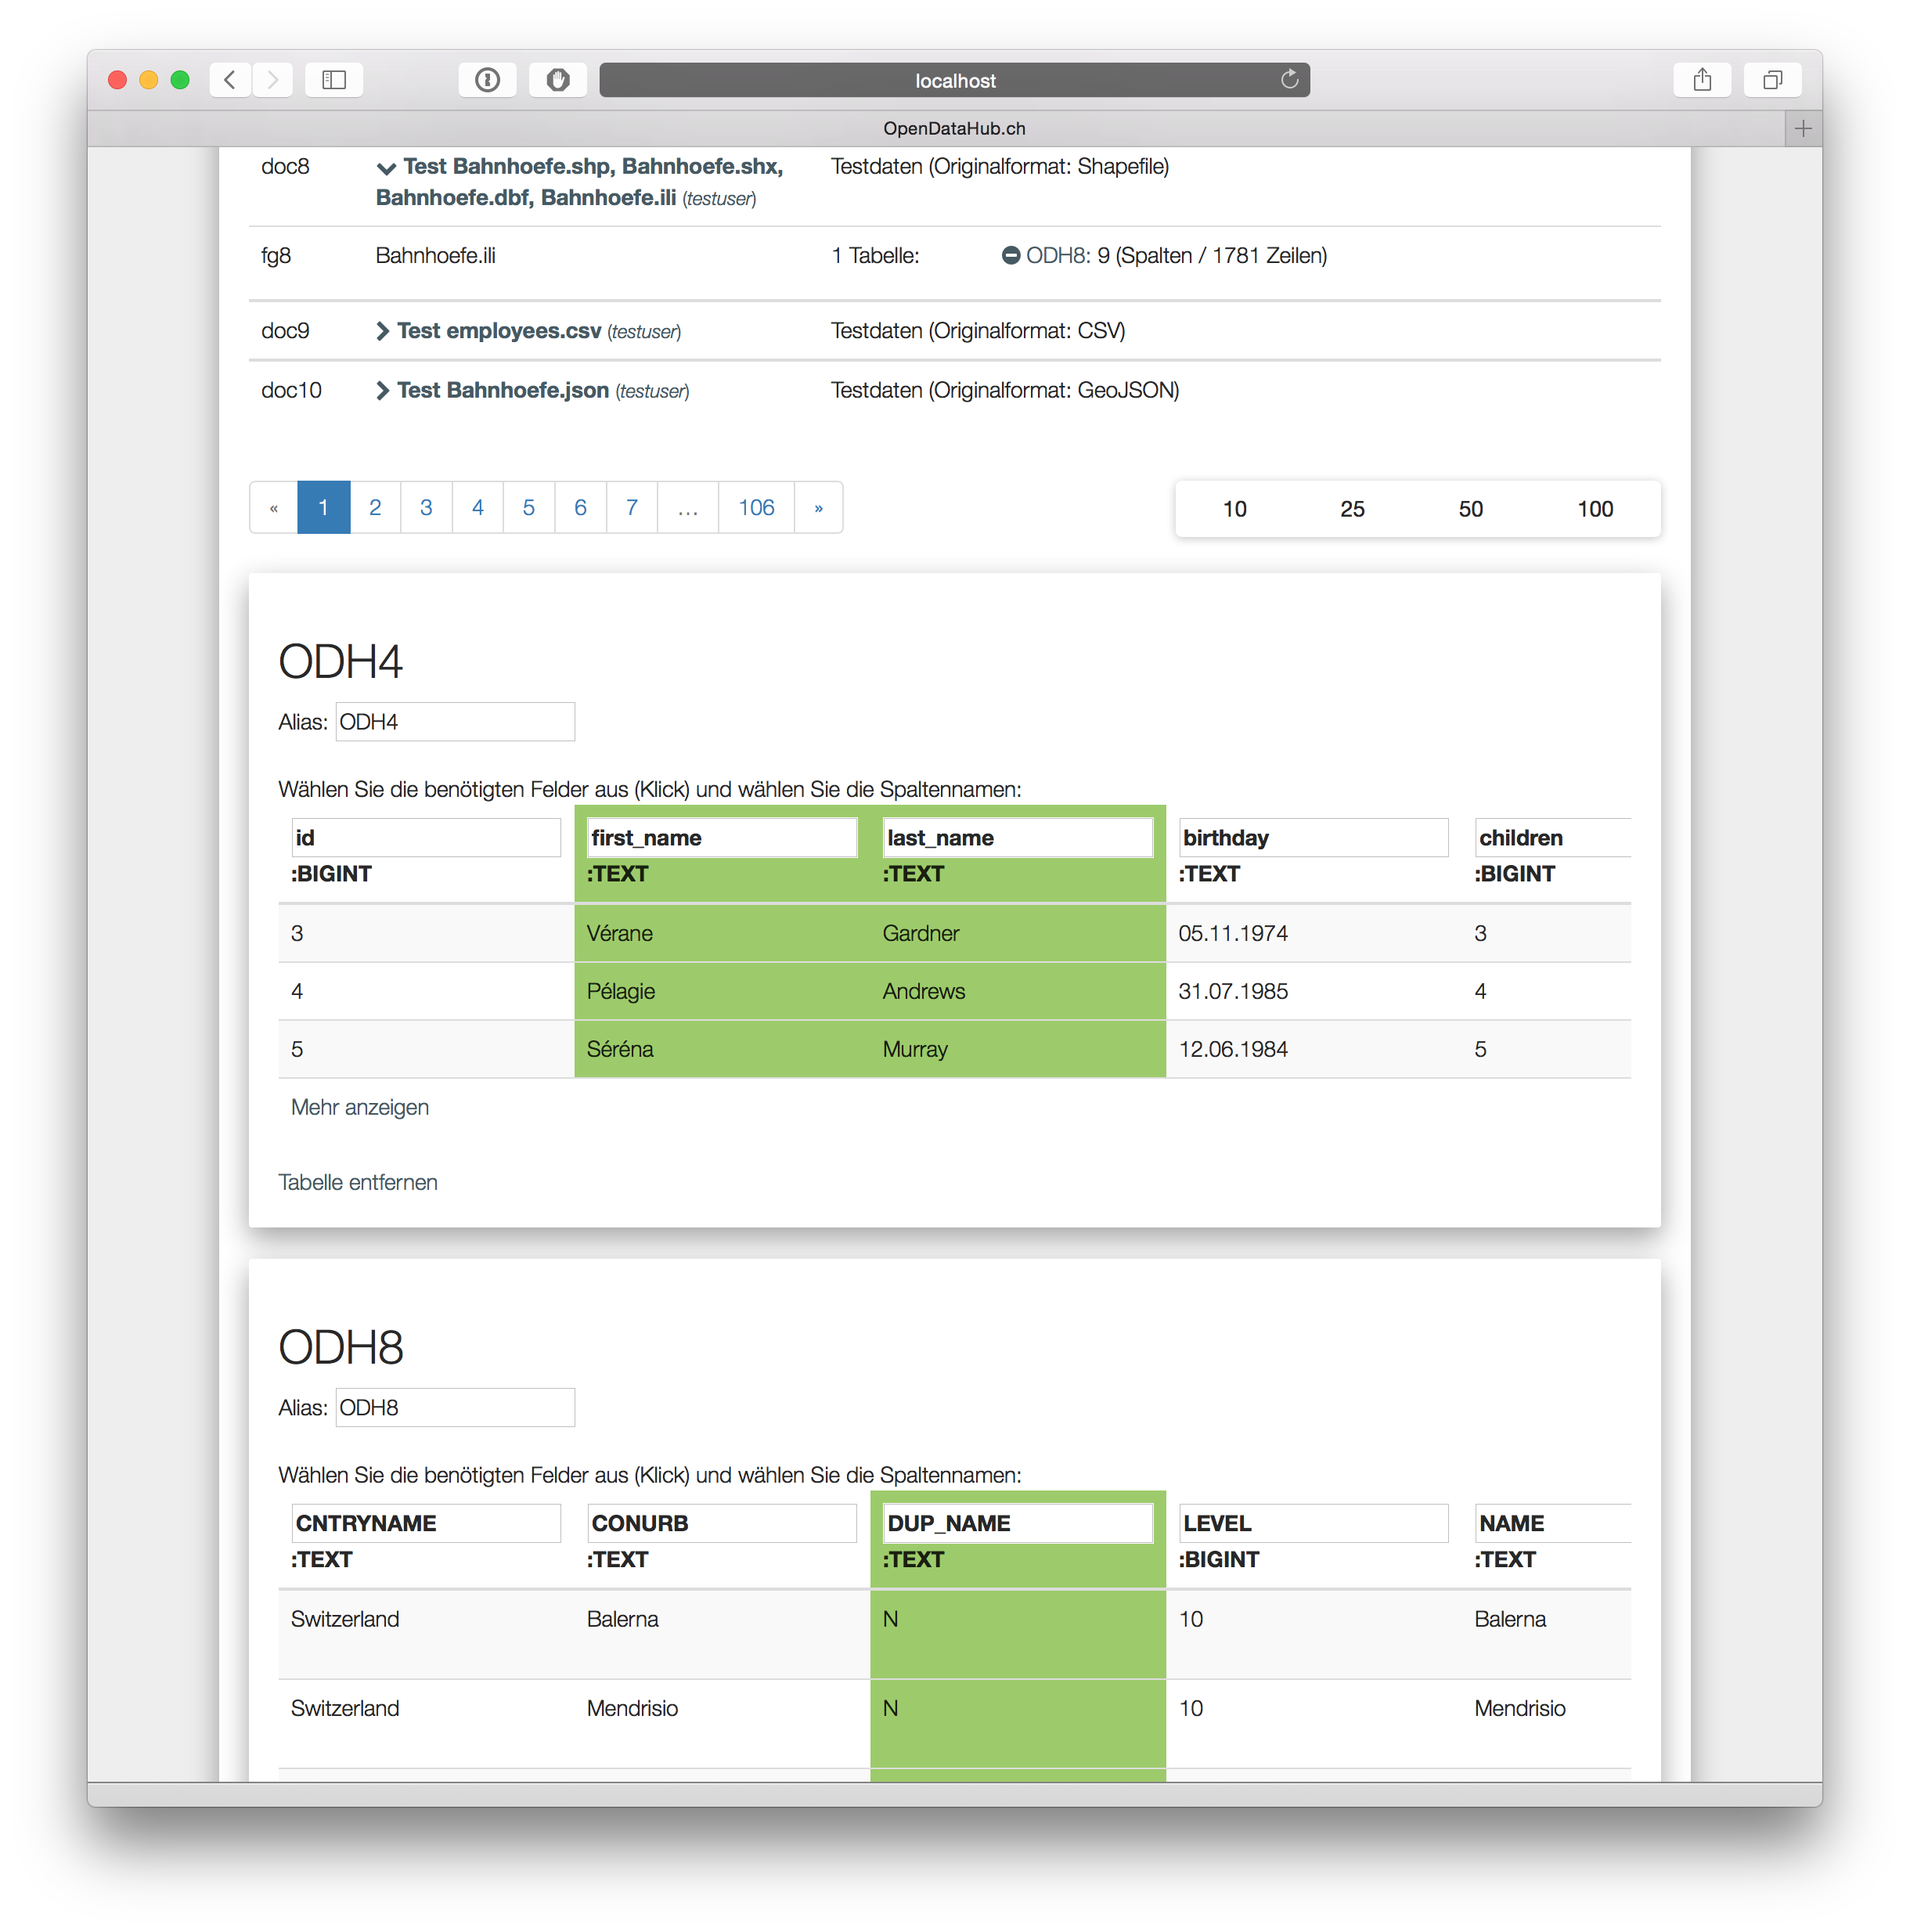
\includegraphics[width=\linewidth]{fig/odhql_wizard_early.png}
\caption{Tabellen können per Klick verbunden werden }
\label{fig:pd:tables_per_click}
\end{figure}
\begin{figure}[H]
\centering
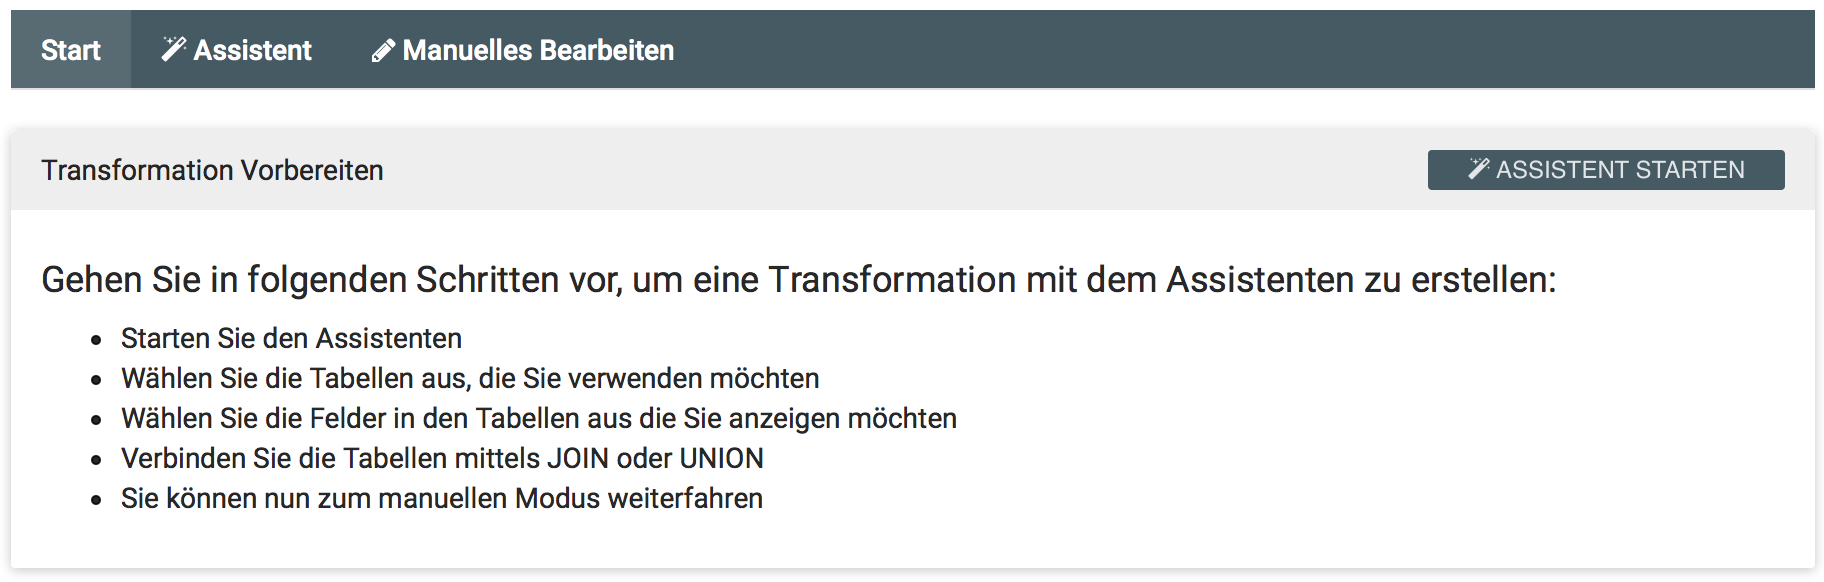
\includegraphics[width=\linewidth]{fig/wizard-step-one.png}
\caption{Einleitung in den Wizard}
\label{fig:pd:wizard-step-one}
\end{figure}
In einem ersten Schritt kann eine Transformation grundlegend erstellt werden. Einfache JOIN und UNION Operationen werden vom Benutzer konfiguriert.
\begin{figure}[H]
\centering
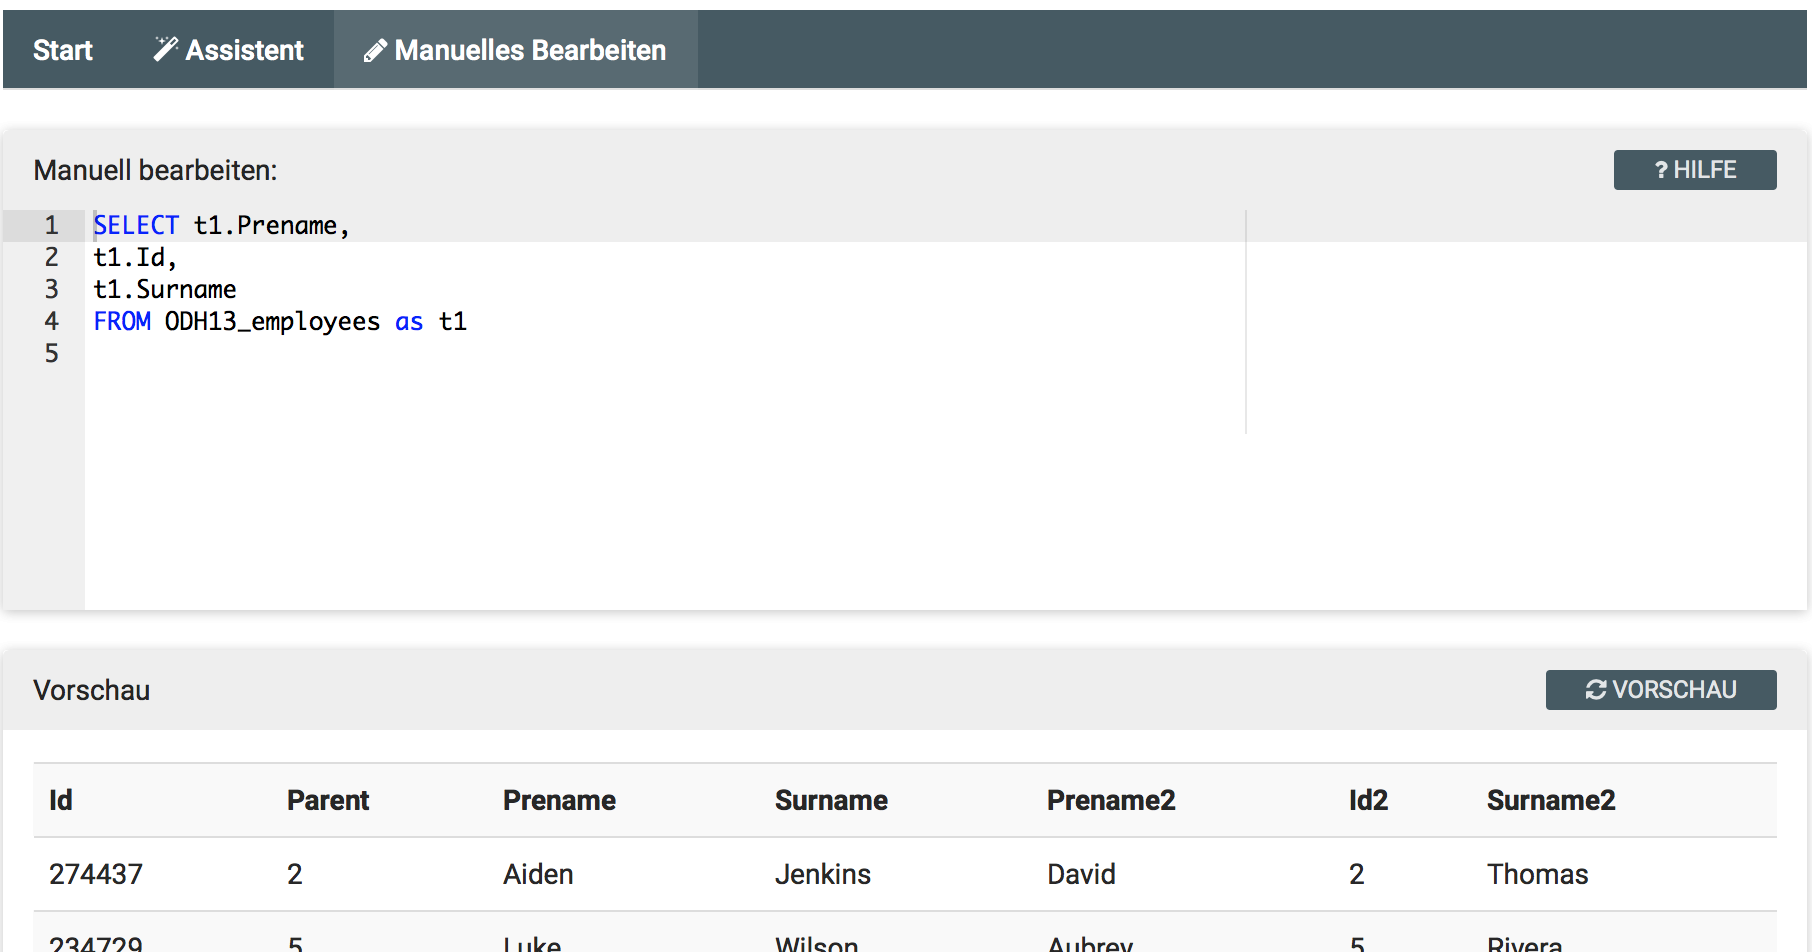
\includegraphics[width=\linewidth]{fig/wizard-manual.png}
\caption{Transformation manuell bearbeiten}
\label{fig:pd:wizard-manual}
\end{figure}

Später können dann die komplexeren Operationen auf die Daten angewendet werden. Hierfür wird der manuelle Modus, in \cref{fig:pd:wizard-manual} beschrieben, verwendet. Im manuellen Modus steht eine Hilfe Seite zur Verfügung, welche sämtliche erweiterten Operationen erklärt.\\
Wird eine Transformation ``als Template'' verwendet, wird beim Speichern keine Prüfung der zugrunde liegenden Daten durchgeführt. So können syntaktisch korrekte, aber noch mit fehlenden Daten belastete Transformationen erstellt werden.

\subsection{Transformationen bearbeiten}
Transformationen können entweder geklont oder überschrieben werden. \cref{fig:pd:transformation-edit} zeigt eine bestehende Transformation, die der angemeldete Benutzer erstellt hat. Beim Klonen legt der Benutzer eine neue Transformation aufgrund der Daten einer Bestehenden Transformation an. Beim Überschreiben kann der Besitzer einer Transformation diese nochmals verändern. Es kann bei diesen Operationen allerdings kein Wizard mehr verwendet werden, da dieser alle manuellen Änderungen überschreiben würde.
\begin{figure}[H]
\centering
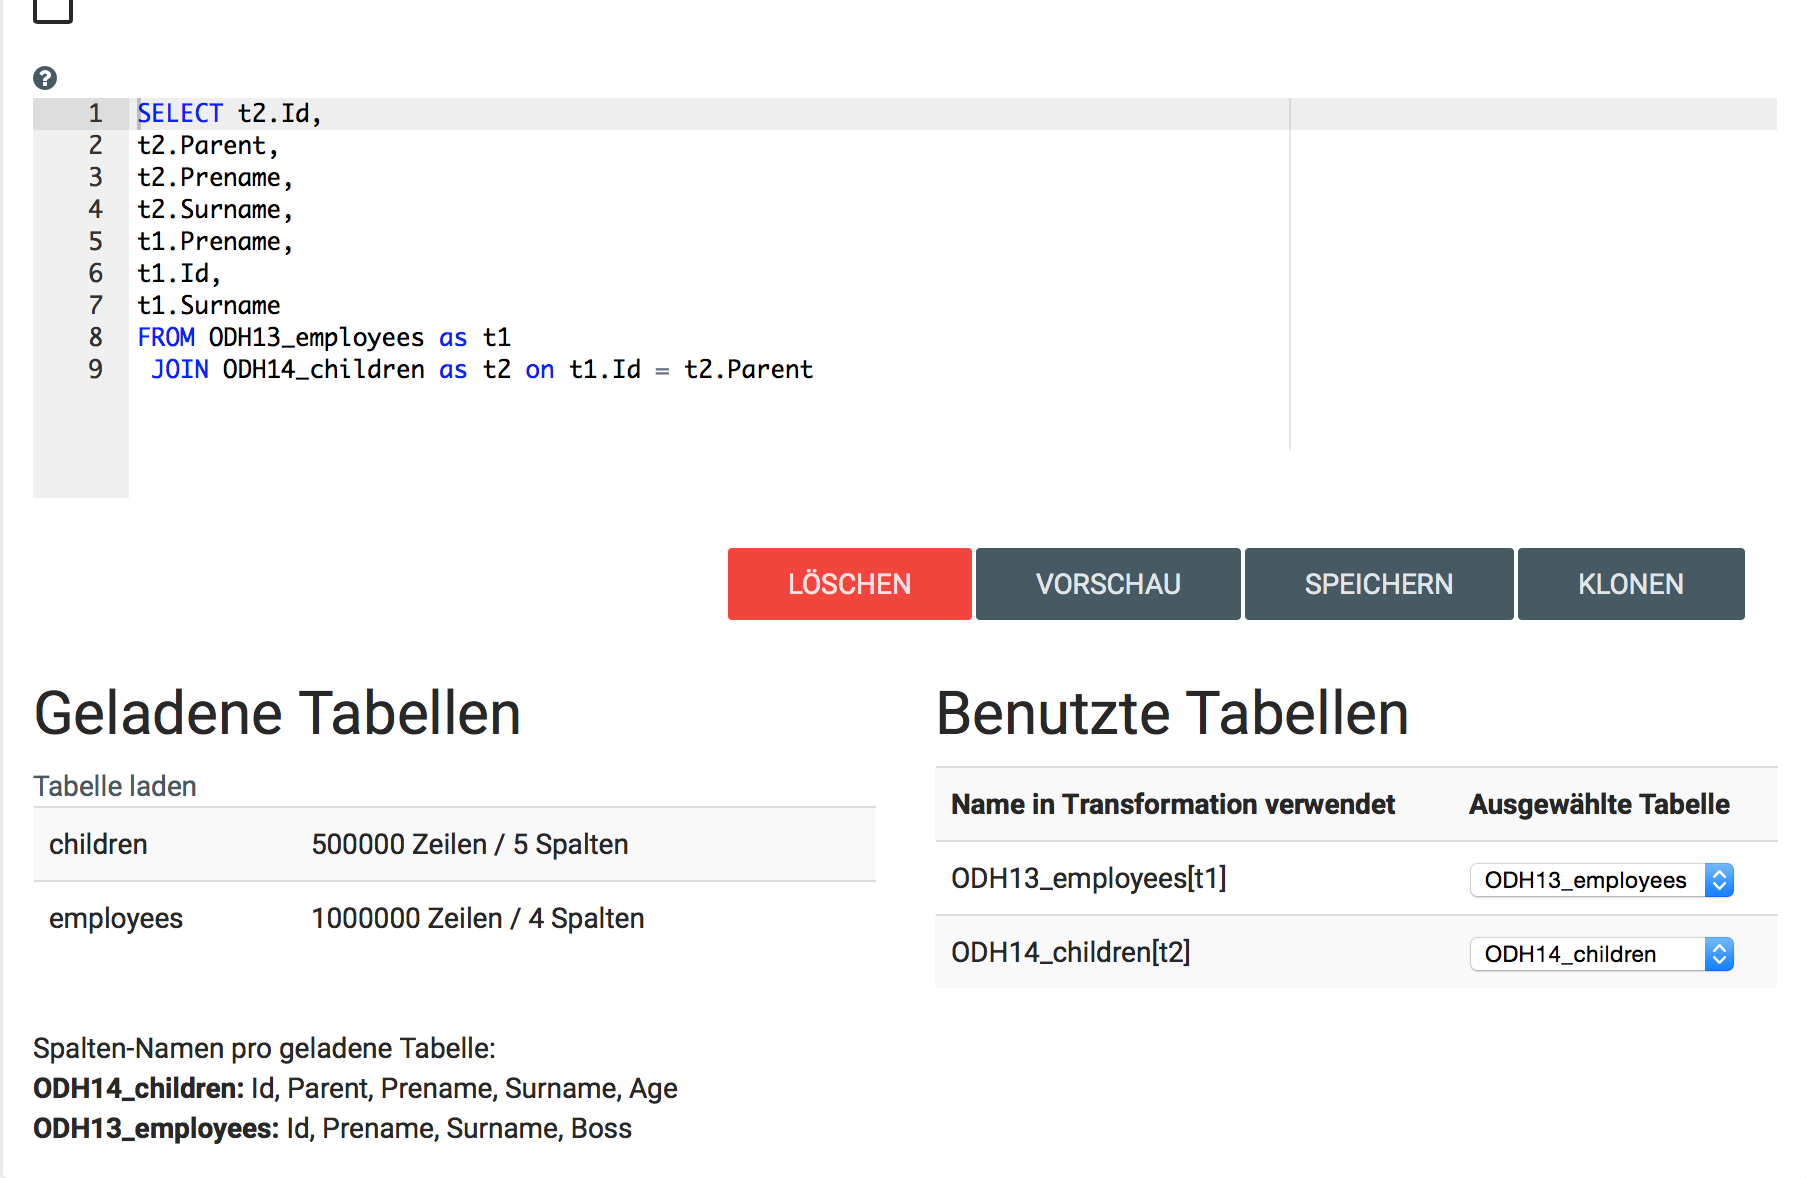
\includegraphics[width=\linewidth]{fig/transformation-edit.png}
\caption{Bestehende Transformation editieren}
\label{fig:pd:transformation-edit}
\end{figure}